\documentclass[12pt]{article}
\usepackage{tabu}
\newcolumntype{A}{D{.}{.}{2.3}}
\usepackage{listings}
\usepackage{graphicx}
\usepackage{booktabs}
\usepackage{float}
\usepackage{hyperref}
\usepackage{caption}
\hypersetup{
	colorlinks=true,
	citecolor=black,
	filecolor=black,
	linkcolor=black,
	urlcolor=black
}
\usepackage{tgbonum}
\graphicspath{ {images/} }
\title{Report on Assignment8 }
\author{Dhaval Limdiwala (173050061) \\ CS-699 \\ IIT Bombay}
\date{October 3 2017}
\pagebreak
% arara: pdflatex: { options: "--jobname 173050062_report" }
\begin{document}
\maketitle
\pagebreak
\tableofcontents
\pagebreak
\pagebreak
\listoffigures
\pagebreak
\section{Top five import and export destinations, by total imports and total exports}
\subsection{Import destnations}
\par {\ttfamily Imports are calculated using {\huge Total value\(INR\)}.}
\par First group by operation on country is performed and and sum aggregate is applied. After that sort is performed and top 5 countries are extracted using head.
Here are top five destinations by total imports

\begin{itemize}
	\item CHINA P RP
	\item U ARAB EMTS
	\item SWITZERLAND
	\item SAUDI ARAB
	\item U S A	
\end{itemize}
\subsection{Export destnations}
\par {\sffamily Exports are calculated using total value\(INR\) using the samew procedure as mentioned above.}
Here are top five destinations b total exports
\begin{itemize}
	\item U ARAB EMTS
	\item U S A
	\item CHINA P RP
	\item SINGAPORE
	\item UNSPECIFIED
\end{itemize}

\begin{figure}[H]
	\centering
	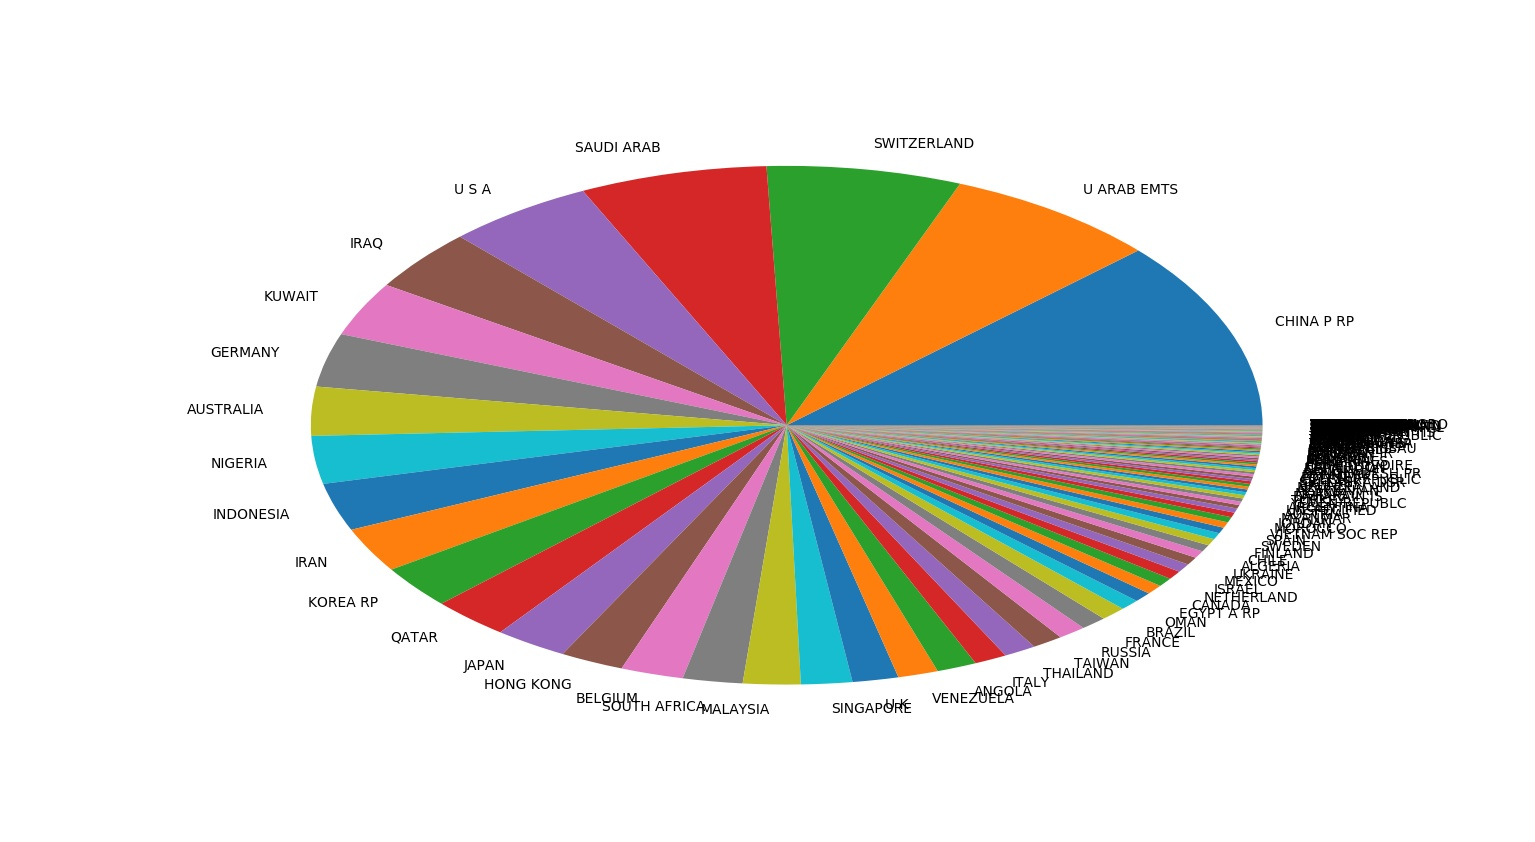
\includegraphics[height=10cm,width=10cm]{image_1.jpg}
	\caption{All countries and their contibution in total imports}
	\label{All countries and their contibution in total imports}
	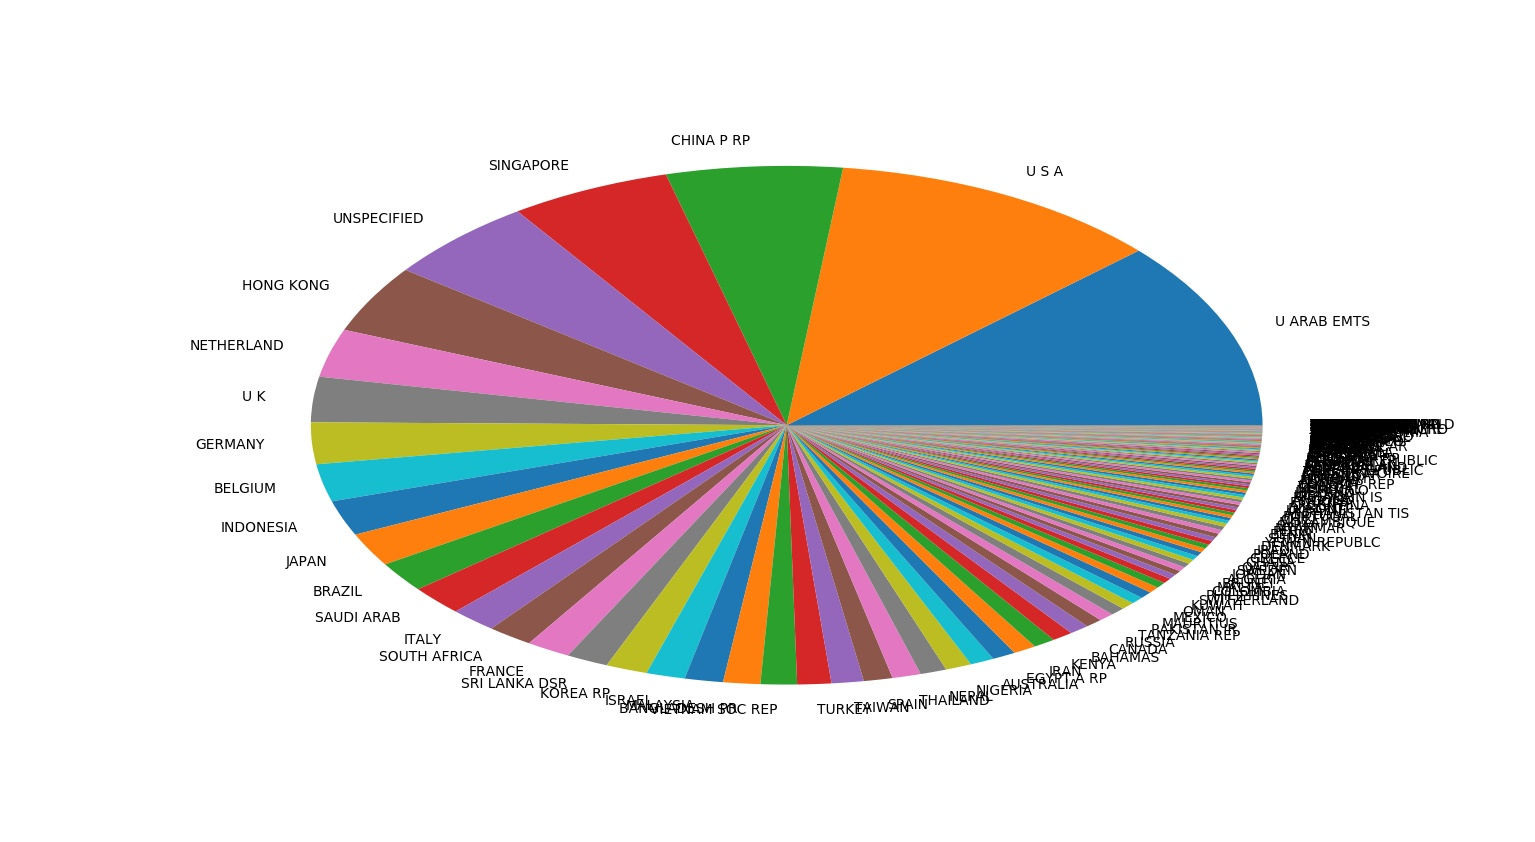
\includegraphics[height=10cm,width=10cm]{image_2.jpg}
	\caption{All countries and their contibution in total exports}
	\label{All countries and their contibution in total exports}
\end{figure}
\pagebreak
\begin{figure}[H]
	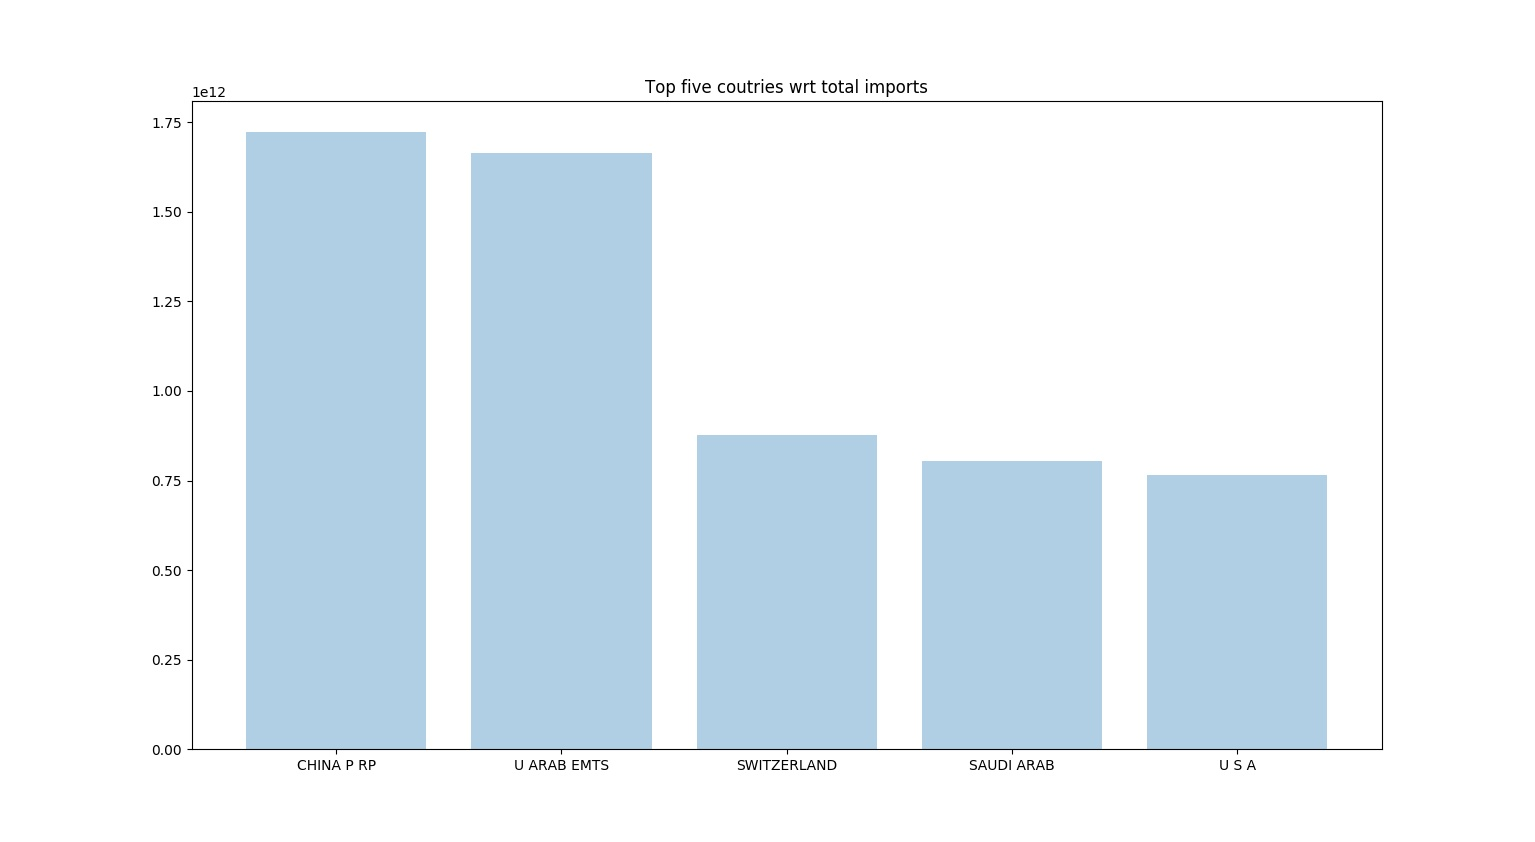
\includegraphics[height=10cm,width=10cm]{image_4.jpg}
	\caption{Top five coutries wrt total Imports}
	\label{Top five coutries wrt total Imports}
	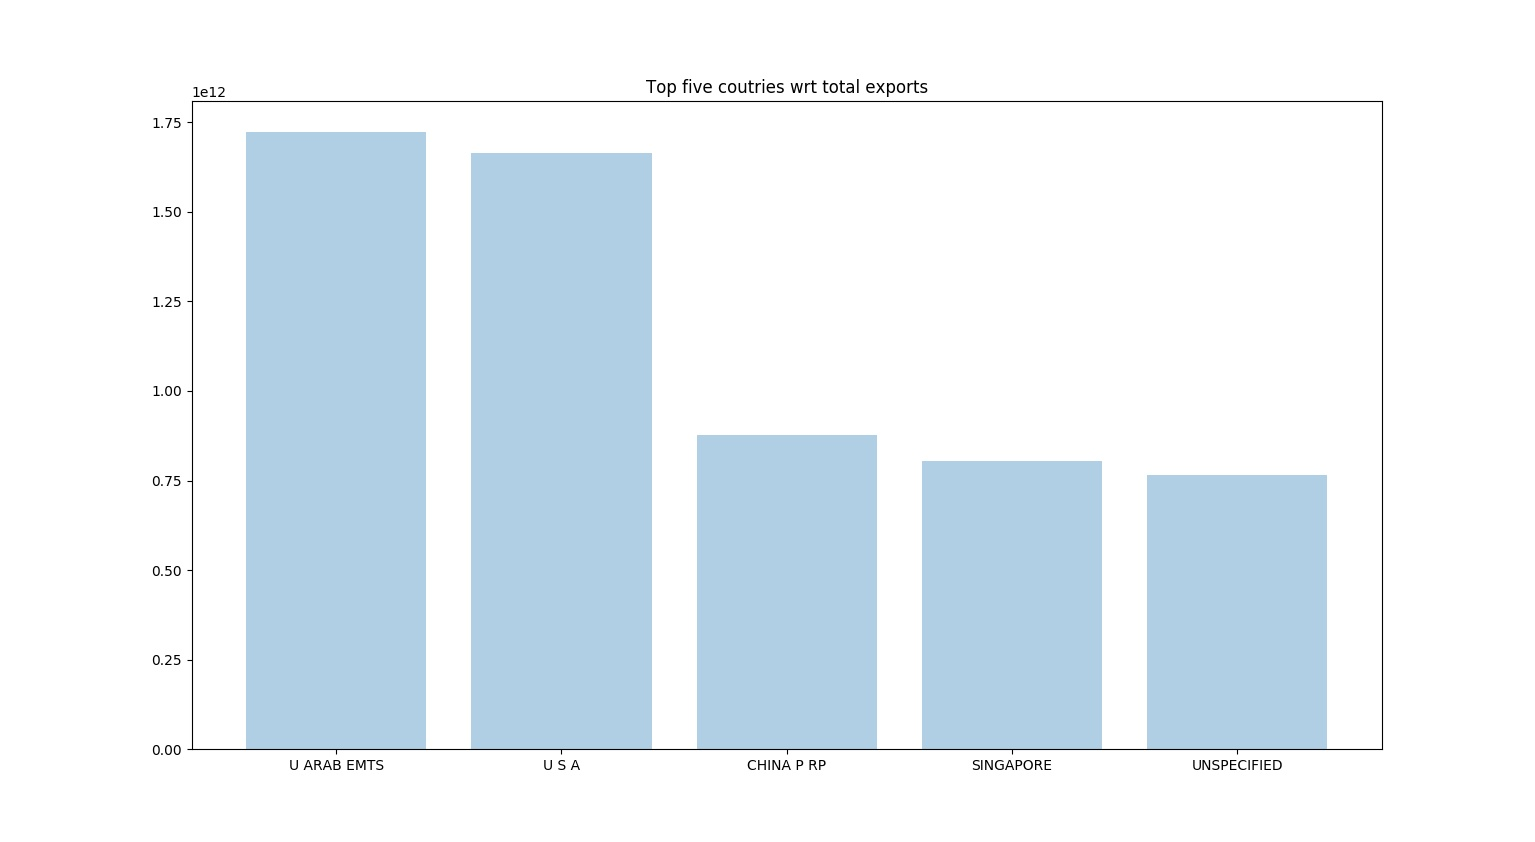
\includegraphics[height=10cm,width=10cm]{image_5.jpg}
	\caption{Top five coutries wrt total Exports}
		\label{Top five coutries wrt total Exports}
\end{figure}
\pagebreak
\section{Top five import and export commodities}
\begin{itemize}
	\item Top five import commodities are
		\begin{enumerate}
			\item PETROLEUM, CRUDE \& PRODUCTS
			\item GOLD
			\item ELECTRONIC GOODS
			\item MACHRY EXCPT ELEC \& ELECTRONIC
			\item PERLS PRCUS SEMIPRCS STONES
		\end{enumerate}


	\item Top five export commodities are
		\begin{enumerate}
			\item PETROLEUM, CRUDE \& PRODUCTS
			\item GEMS \& JEWELLARY
			\item TRANSPORT EQUIPMENTS
			\item OTHER COMMODITIES
			\item MACHINERRY AND INSTRUMENTS
			
		\end{enumerate}
\end{itemize}


\pagebreak
\section{All countries to whom our export is more than Rs 10,000 Cr using query method}
\begin{tabular}{lrr}
\toprule
{} &        exports &       imports \\
\midrule
AUSTRALIA       &   119902198011 &  7.130386e+11 \\
BAHAMAS         &   105614860388 &  1.568729e+08 \\
BANGLADESH PR   &   183867403716 &  2.792558e+10 \\
BELGIUM         &   342080841360 &  5.000279e+11 \\
BRAZIL          &   275768826842 &  2.065963e+11 \\
CHINA P RP      &   876693687587 &  2.759986e+12 \\
EGYPT A RP      &   117357337775 &  1.438294e+11 \\
FRANCE          &   220219207138 &  2.084836e+11 \\
GERMANY         &   379817399877 &  7.809529e+11 \\
HONG KONG       &   618772346350 &  5.071798e+11 \\
INDONESIA       &   321007511450 &  6.975913e+11 \\
IRAN            &   115118034607 &  6.544814e+11 \\
ISRAEL          &   193326493427 &  1.240863e+11 \\
ITALY           &   232826478090 &  2.596234e+11 \\
JAPAN           &   305195206178 &  5.814288e+11 \\
KENYA           &   109873301637 &  5.655950e+09 \\
KOREA RP        &   207814242260 &  6.290300e+11 \\
MALAYSIA        &   191032438347 &  4.578630e+11 \\
NEPAL           &   131302514781 &  2.639361e+10 \\
NETHERLAND      &   439137717400 &  1.294779e+11 \\
NIGERIA         &   130514071726 &  6.979970e+11 \\
SAUDI ARAB      &   272081981668 &  1.493500e+12 \\
SINGAPORE       &   803632863320 &  4.073224e+11 \\
SOUTH AFRICA    &   227296847495 &  4.765721e+11 \\
SPAIN           &   143687856091 &  8.632672e+10 \\
SRI LANKA DSR   &   209514580130 &  3.435715e+10 \\
TAIWAN          &   159861741400 &  2.470947e+11 \\
THAILAND        &   142535348805 &  2.578748e+11 \\
TURKEY          &   168940115453 &  4.437597e+10 \\
U ARAB EMTS     &  1722684826477 &  1.711266e+12 \\
U K             &   413240885916 &  3.662315e+11 \\
U S A           &  1664743129673 &  1.172933e+12 \\
UNSPECIFIED     &   764565004286 &  5.018599e+10 \\
VIETNAM SOC REP &   180849830415 &  8.373222e+10 \\
\bottomrule
\end{tabular}


\pagebreak
\section{Creating a new table with column headings "Country", "Transaction", "Value" from table in answer 5 using melt mothod}
\begin{tabular}{lllr}
\toprule
{} &      Country & Transaction &         Value \\
\midrule
39 &   CHINA P RP &     Imports &  2.759986e+12 \\
29 &  U ARAB EMTS &     Exports &  1.722685e+12 \\
63 &  U ARAB EMTS &     Imports &  1.711266e+12 \\
31 &        U S A &     Exports &  1.664743e+12 \\
55 &   SAUDI ARAB &     Imports &  1.493500e+12 \\
65 &        U S A &     Imports &  1.172933e+12 \\
5  &   CHINA P RP &     Exports &  8.766937e+11 \\
22 &    SINGAPORE &     Exports &  8.036329e+11 \\
42 &      GERMANY &     Imports &  7.809529e+11 \\
32 &  UNSPECIFIED &     Exports &  7.645650e+11 \\
\bottomrule
\end{tabular}


\pagebreak
\section{Commodities that we both export and import}
\begin{tabular}{lrr}
\toprule
{} &       Exports &       Imports \\
Commodity                      &               &               \\
\midrule
COMP.SOFTWARE IN PHYSICAL FORM &  4.666247e+10 &  1.050293e+11 \\
COTTON RAW INCLD. WASTE        &  4.143706e+11 &  3.523719e+10 \\
COTTON YARN \& FABRICS          &  7.350993e+11 &  2.776343e+10 \\
ELECTRONIC GOODS               &  8.630141e+11 &  3.276628e+12 \\
HANDLOOM PRODUCTS              &  5.443871e+10 &  1.089359e+09 \\
MACHINE TOOLS                  &  3.879292e+10 &  2.933595e+11 \\
MANUFACTURES OF METALS         &  1.005158e+12 &  4.375569e+11 \\
NON-FERROUS METALS             &  3.665418e+11 &  5.130657e+11 \\
OTHER CEREALS                  &  1.371015e+11 &  1.406401e+09 \\
OTHER COMMODITIES              &  1.453747e+12 &  1.720925e+12 \\
PETROLEUM, CRUDE \& PRODUCTS    &  5.955936e+12 &  1.663531e+13 \\
PROJECT GOODS                  &  9.588092e+09 &  7.790110e+11 \\
PULSES                         &  2.345744e+10 &  2.166988e+11 \\
SPICES                         &  2.853915e+11 &  4.780713e+10 \\
SUGAR                          &  1.734298e+11 &  3.385539e+10 \\
TEA                            &  8.755605e+10 &  4.933388e+09 \\
TRANSPORT EQUIPMENTS           &  2.014760e+12 &  1.420874e+12 \\
WHEAT                          &  1.151162e+11 &  6.112098e+07 \\
\bottomrule
\end{tabular}


\pagebreak

\section{Random content}

Here are formulas for gaussian distribution.
\begin{equation}
	F (x) = \frac{1}{\sigma \sqrt {2\pi}}e^{\frac{ - \left( {x - \mu } \right)^2}{2\sigma^2}}
\end{equation}
where,
\begin{equation}
	\mu = \frac{1}{N}\sum_{i = 1}^{N}x_i
\end{equation}
\begin{equation}
	\sigma^2 = \frac{1}{N}\sum_{i=1}^{N}(x_i - \mu)^2
\end{equation}

Here, is the histogram which decribes above gaussian distribution
\begin{figure}[H]
\centering
	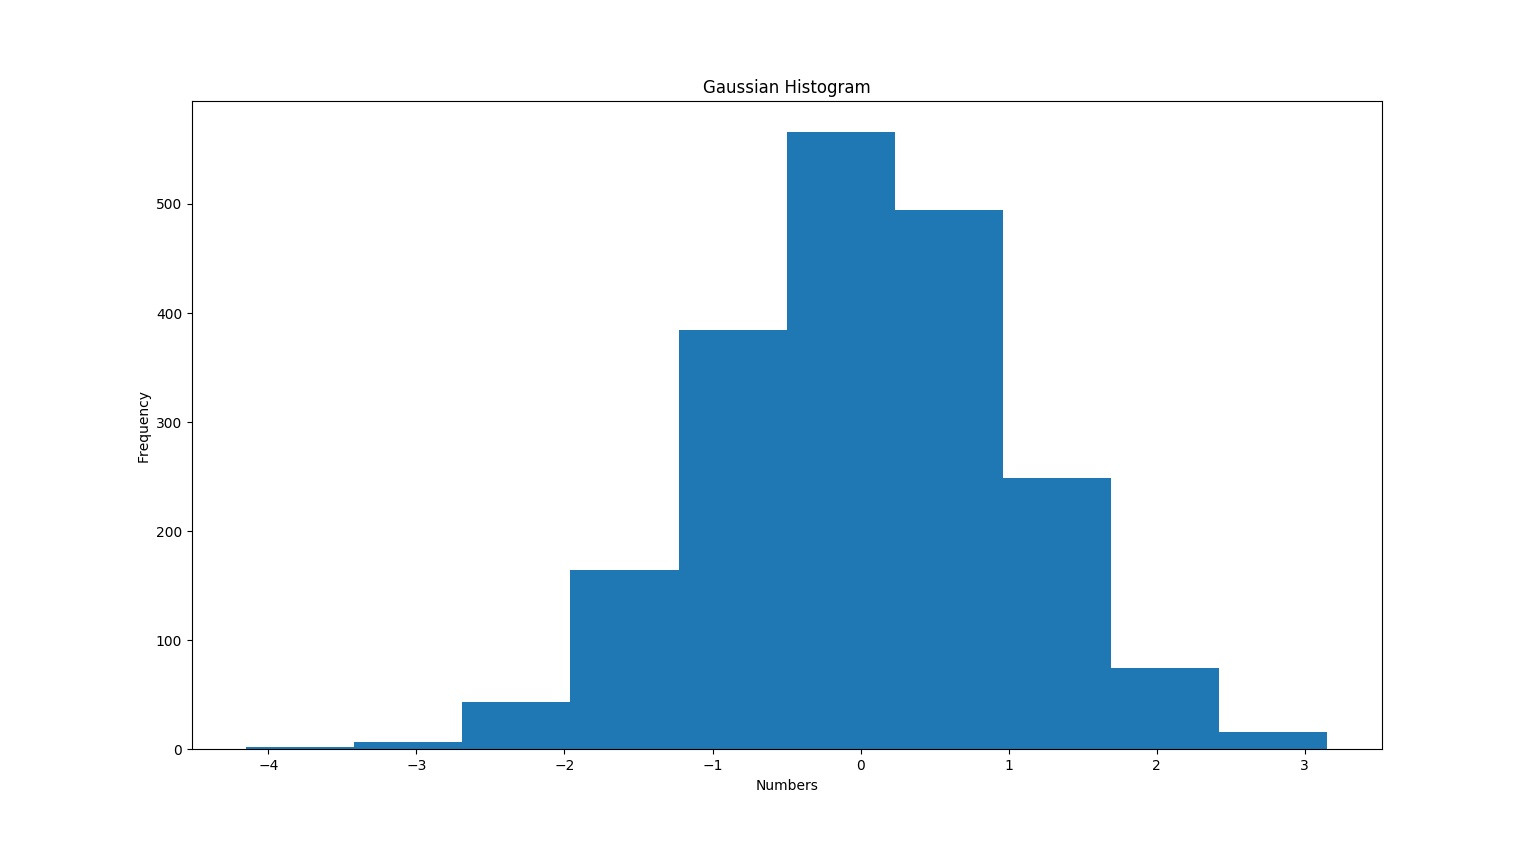
\includegraphics[height=10cm,width=10cm]{image_3.jpg}
	\caption{Gaussian histogram}
	\label{Gaussian histogram}
\end{figure}



Some more random Line Charts
\begin{figure}[H]
	\centering
	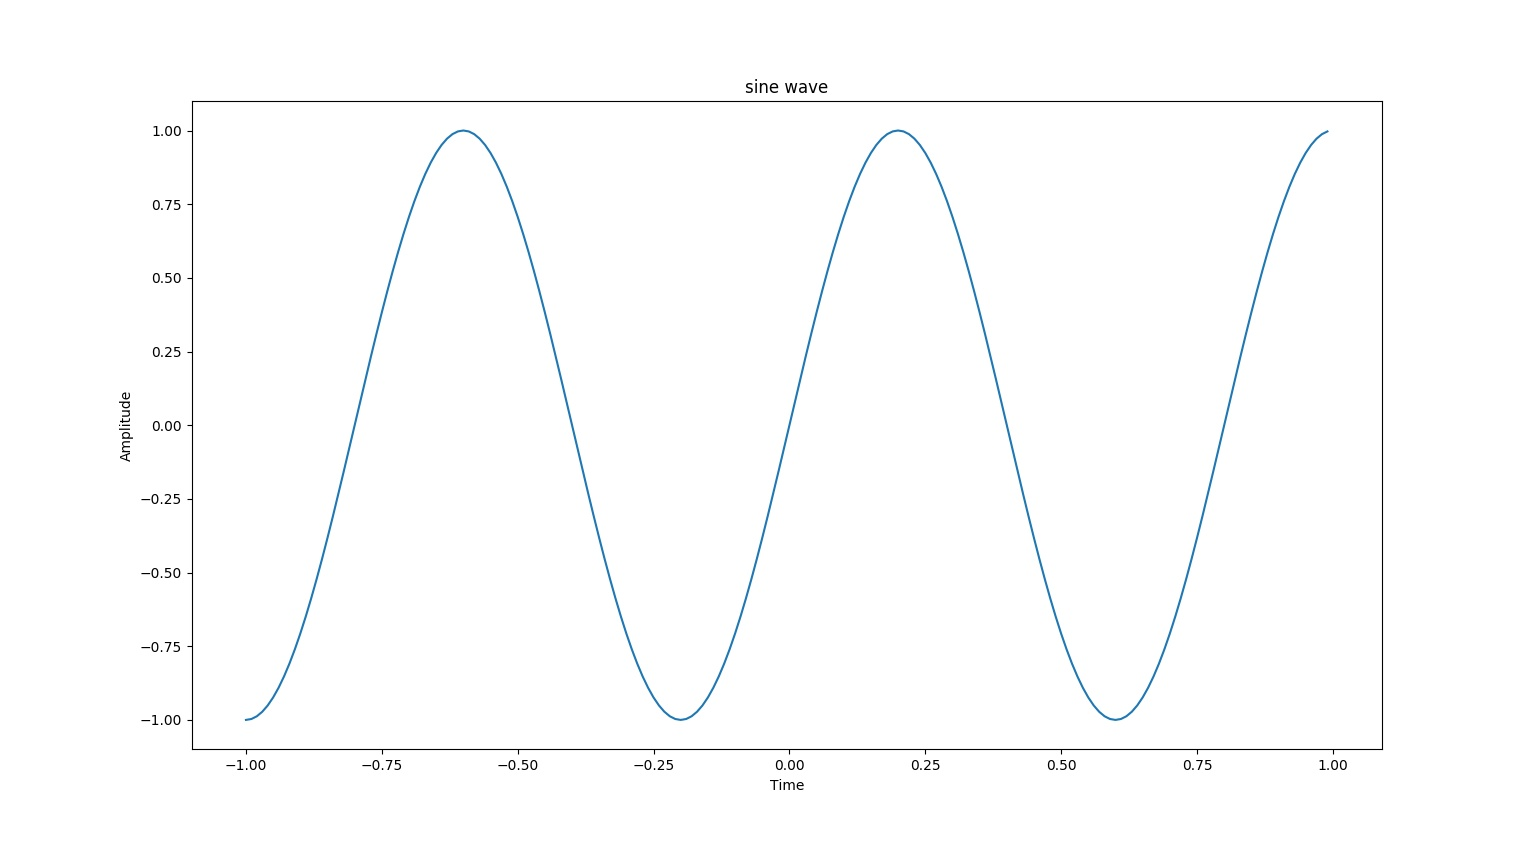
\includegraphics[height=10cm,width=10cm]{image_6.jpg}
	\caption{Sine wave}
	\label{Sine wave}
	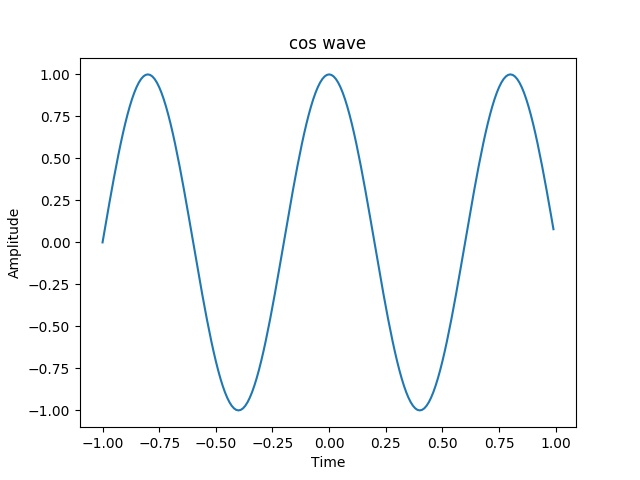
\includegraphics[height=10cm,width=10cm]{image_7.jpg}
	\caption{Cos wave}
	\label{Cos wave}
\end{figure}

Some more formulas
\\ \\ \\
Binomial distribution
\begin{equation}
	f(k;p) = p^k(1 - p)^{1-k} .....for k \in (0,1)
\end{equation}

Beta distribution
\begin{equation}
	PDF = \frac{x^{\alpha - 1}(1 - x)^{\beta - 1}}{B(\alpha,\beta)}.....where B(\alpha,\beta) = \frac{\Gamma(\alpha)\Gamma(\beta)}{\Gamma(\alpha + \beta)}
\end{equation}
\end{document}